%
% Copyright (C) 2012 Jan Nowotsch
% Author Jan Nowotsch	<jan.nowotsch@gmail.com>
%
% Released under the terms of the GNU GPL v2.0
%



\section{Bridge Driver}
	The bridge device driver family provides the possibility to connect leaf nodes in the device tree, e.g. a uart and an i2c device. Beneath others, this allows to transfer data between otherwise incompatible protocols.

	\subsection{Device Tree Configuration}
		To connect two device tree nodes they need to provide an interface to one of the bridge adapters. Bridge adapters provide the interface between a bridge and the target protocol.
		As an example Listing~\ref{lst:brdg_uart_term} shows a device tree excerpt that connects an avr uart \lstinline{uart0} with a terminal \lstinline{ttybrdg0}.

		\begin{lstlisting}[label={lst:brdg_uart_term},caption={Bridge example: uart to terminal bridge.}]
uart0 = {
	compatible = "avr,uart";
	...

	brdg0-left = {
		compatible = "bridge,uart-itf";
		...
	};
};

brdg0-right = {
	compatible = "bridge,uart-dev";
	...

	ttybrdg0 = {
		compatible = "terminal";
		...
	};
};
		\end{lstlisting}

		As another example, Listing~\ref{lst:brdg_uart_i2c} shows how to connect a uart and an i2c device.

		\begin{lstlisting}[label={lst:brdg_uart_i2c},caption={Bridge example: uart to i2c bridge.}]
uart0 = {
	compatible = "avr,uart";
	...

	brdg0-left = {
		compatible = "bridge,uart-itf";
		...
	};
};

i2c0 = {
	compatible = "avr,i2c";
	...

	brdg0-right = {
		compatible = "bridge,i2c-itf";
		...

	};
};
		\end{lstlisting}

		The link between two bridge ends is established through the bridge id, which is part of the bridge configuration in the device tree.

	\subsection{Bridge Protocol}
		The bridge protocol is split into three parts, the header, payload and checksum. The header bytes are transfered one byte at a time, expecting an acknowledgment after each transfer. A byte is acknowledged by sending back its inversion. The payload is transfered in chunks, whereas only the last byte of a chunk is expected to be acknowledged. The size of chunks is specific to each bridge and can be configured through the device tree. Finally, the checksum is a single byte, which also needs to be acknowledged. The checksum is computed based on the payload according to $csum_{i + 1} = csum_i + (\sim data[i]) + 1$ with $csum_0 = 0$.

		Figure~\ref{fig:brdg_protocol} summarises the read and write sides of the protocol.

		\begin{figure}[h]
			\centering	
			\includegraphics[scale=.75]{driver/bridge/protocol}
			\caption{Bridge protocol.}
			\label{fig:brdg_protocol}
		\end{figure}
